\documentclass[10pt,a4paper]{article}
\usepackage[utf8]{inputenc}
\usepackage{amsmath}
\usepackage{amsfonts}
\usepackage{amssymb}
\usepackage{graphicx}
\usepackage{framed}
\usepackage{float}
\usepackage{hyperref}
\author{Paul Cowie \and Jacob Ford \and Nicole Munro \and William Kavanagh \and Ben Procter \and Pregashni Mohanarajah }
\date{}
\title{Team Six: IS(H) AX2, Report 2}
\begin{document}
\maketitle

\section*{Introduction}

Our application, 120 Degrees, offers users an experience unmatched by any other currently available. Through the use of a multidimensional query matrix, our application allows users to rank restaurants in their vicinity based on multiple axes simultaneously. The power of our application comes from the pairing of very basic, yet functional interaction from the user generating results that are highly specific to their needs. This advanced functionality is all provided with in a polished, professional product that is pleasing to the eye without any superfluous visual flair obstructing user-interaction.

The main element of our product that makes us stand out is how we deal with user search querying. By allowing multiple, weighted queries that can be deemed either positive or negative we can deliver much more precise suggestions that competitors much earlier in a user’s usage cycle. There are not many other services which allow users to negatively mark certain aspects of a restaurant in the way we do and this allows us to remove several suggestions in which the user would have no interest. The truth is that what users specifically do not want is as important as what they do. In an ever growing and highly competitive market such as this, sifting through the vast quantity of offers efficiently can only be done if users can specify the negative attributes that they find the most undesirable alongside what is most important to them. Searching for everything simultaneously also makes our service significantly more efficient for our users relative to the key competitors, and all without sacrificing any of the functionality offered by competitors. Speed and efficiency are two metrics which have become even more important than they were before in the current climate in which the everyday consumer is more tech-savvy than ever before. The ranking of queries is also a feature unique to 120 degrees that results in users getting personalised results. The services currently available will allow for searching by a single cuisine, whereas with 120 degrees users can search for multiple at a time and rank them by preference “I really want Indian, but I wouldn’t mind getting pizza” - this form of query is possible with 120 degrees in a single search, functionality that is not offered by any services currently on the market. Through our unique approach to searching users will get a service that is more efficient, more personalised and more accurate than the currently available applications offering similar services.

Another element of our design which allows for users to obtain suggestions more highly tuned to their specifics needs is the ability to search for literally any term they can think of - There are not many other services which allow users to search for how “swanky” or “ambient” a restraunt is. This is another example of unique functionality that our application provides whilst also keeping an intuitive design that all users will be able to understand in mere moments. In designing the application we wanted to ensure we catered to every need and from a discussion on this topic we had the idea to allow users to search for absolutely everything, thereby ensuring all of their needs were catered to. This functionality also means that we have not designed our product for a specific user-group in mind, it caters to everyone. Paired with an attractive, but understated visual design, this functionality ensures no-one will feel that they are not the intended audience for the product.

We worked very hard when building this product to ensure that functionality was not sacrificed for simplicity and vice-versa. This endeavour has left us with a product that is as easy to use as any currently available, but one that we believe will generate more specific results than any other currently available. The way in which our results are displayed was designed to best incorporate the associative ranking we give each restaurant, whilst also being both attractive and distinctive, a way to visually set our product apart from others. This distinctiveness is something we strongly believe we have achieved by displaying our results as tessellating hexagons which can expand to give more detailed information about a restaurant and which is coloured to distinguish the correlation to the user’s multidimensional query.

Our product offers all of the key elements offered by similar applications, whilst also expanding on them to give users more control of the suggestions that are generated. It uses user’s location data to search by distance, it allows for searching by cuisine, price and average rating, whilst for the first time allowing users to search by these criteria concurrently, making for a much more streamlined, smoother process. All of this, in addition to being able to search for custom queries and assigning weight to any given query, delivered in a professional and intuitive environment, puts our product to the forefront of it’s field. 

\section*{Briefing to the City Council}

\section*{Design Requirements}

From the original concept, we set out with the aim of designing an interface that would allow users to search various ‘keywords’ allowing them to choose the categories that they have the highest/lowest preference to.

\begin{figure}[H]
	\begin{center}
		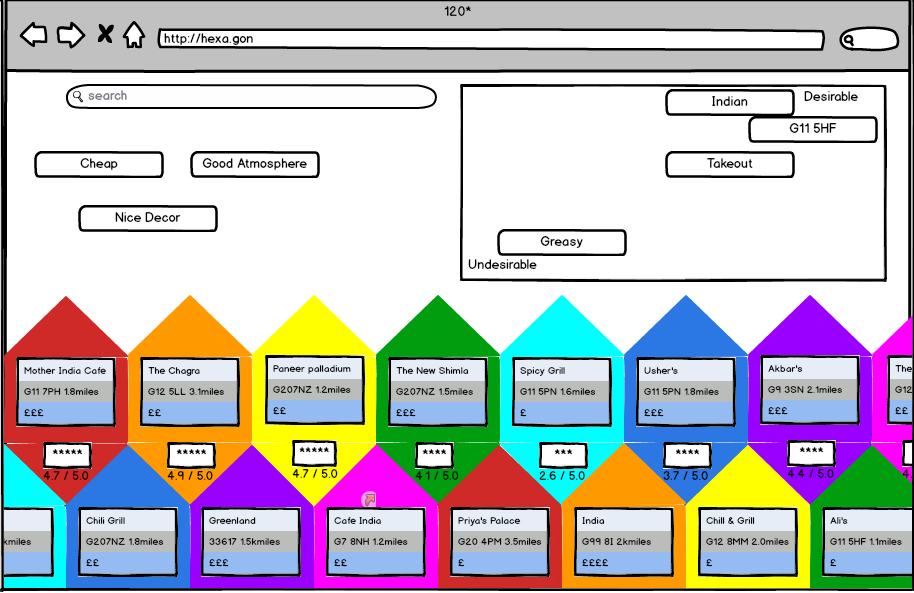
\includegraphics[scale=0.37]{Screenshot.png}
		\caption{Paper prototype of design}
		\label{figure:prototype}
	\end{center}
\end{figure}


We were able to achieve this through its incorporation into the pinboard system where choices were split between cuisine types and other metrics such as ‘Nut-Free’ or ‘Expensive’. We also allowed the users the create their own if there were options that had not been taken into consideration.

\begin{figure}[H]
	\begin{center}
		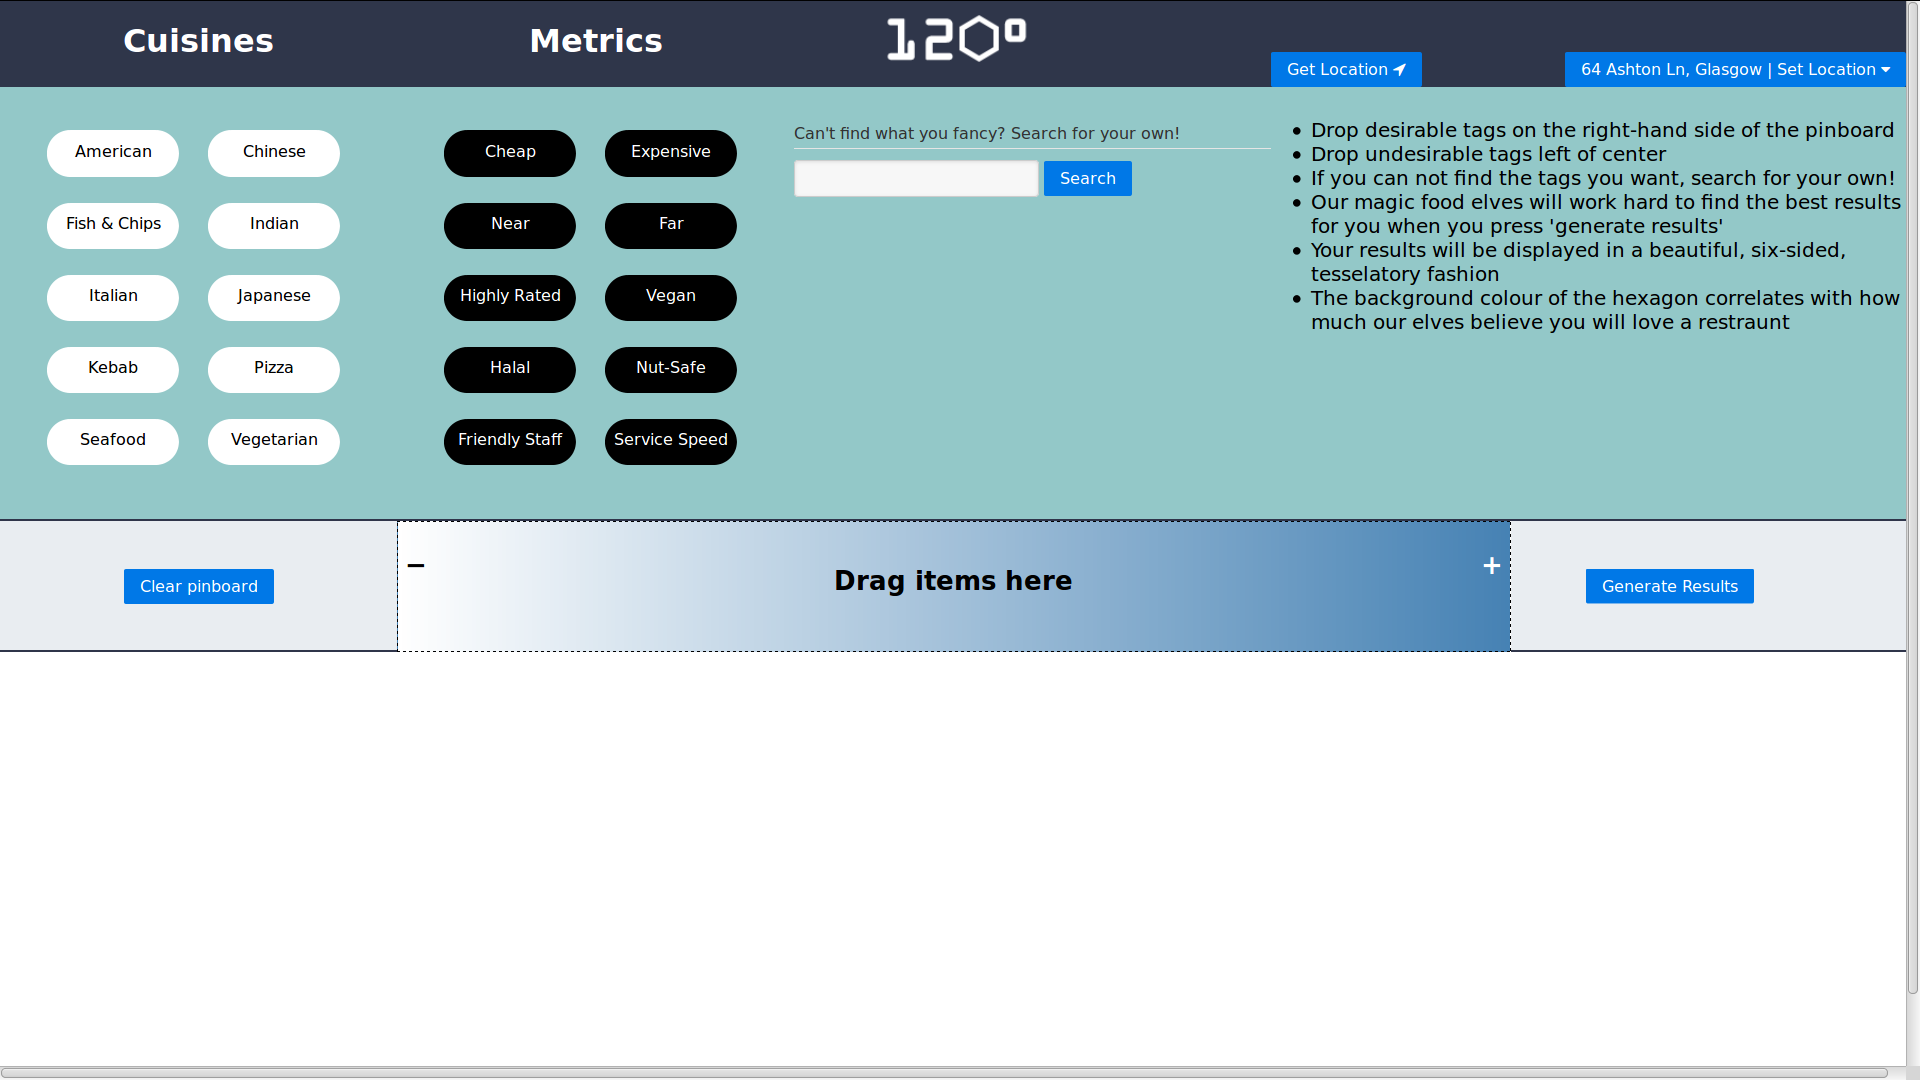
\includegraphics[scale=0.2]{newScreenshot.png}
		\caption{Finished design without results}
		\label{figure:finished-design-no-results}
	\end{center}
\end{figure}

One of the key features of our design was that the results were to be displayed in a iconic hexagonal design. Originally, the plan was to have the hexagons tessellating across the screen in a variety of different covers. However, as the design process went on, we made the team decision that it would make more sense to have a gradient colour scheme which gets paler the worse the result matched the query. This can be seen in Figure \ref{figure:finished-design-no-results} whereas the hexagons go from left to right starting on the top left and finishing at the right of the bottom row, the shade of steel blue gradually gets fainter and fainter.

In the original concept, the pinboard concept was to have the design running from bottom left to top right representing the least desirable to the most respectively. However, over time due to time constraints and also to make better use of the whole screen, we chose that it would make more sense to make the pinboard operate purely on a 2-D Axis where preference towards certain tags was determined by its location on the x-axis with preference increasing the further to the right of the axis a tag was placed by the user.

The decision was also taken to move the pinboard from the top of the screen to the centre. This was due to its ability to created a divider between the searching components at the top of the page and the hexagonal results that are generated and displayed below.

\section*{Submission Description}

Many of the original design decisions carried through to the final product. Our key features - the multitude of tags, the highly interactive pinboard, and the use of hexagons to display results - are all present in the final product. They have all experienced minor changes to better suit the formatting of the website and the data - the pinboard is now completely horizontal and resides in the middle of the screen, while the search bar and suggested tags occupy the top third. The hexagons also display slightly different data based on the results returned by the Google Places API. We also included several new features, including a map for the user to choose their location and tips for effective use. The multi-dimensional search algorithm was largely implemented as envisioned, but some Google Places API limitations prevented the idea to be explored in full.

However, several pieces of functionality were ultimately not included. One feature that did not make it to the final product was the idea that the hexagons would update as the user dragged tags to the pinboard. This was scrapped due to the complexity of the algorithm and the amount of data being sent to and returned from the Google Places API to generate the best results possible. In addition, due to the required queries, fewer results are displayed than originally intended, with many being truncated by the limit on the number of queries one webpage can request of Google. We decided to keep the result count low to allow for higher-quality results that best match the search terms.

\section*{Analytical Findings}
\subsection*{Investigation 1}

The first investigation measured the amount of time that it takes for a user to enter tags they want and get results. To ensure that the tags used matched real-world usage, some repeatable, representative tasks were devised.

\begin{itemize}
	\item \textbf{Task 1:} Search for cheap, nearby Italian food.
	\item \textbf{Task 2:} Change location to their home, then search for Chinese or Thai food, but not Japanese
	\item \textbf{Task 3:} Search for kosher food that isn’t American
\end{itemize}

The results are shown in Table \ref{table:experiment-1}.

\begin{table}[H]
\centering
\begin{tabular}{c|ccc|}
\cline{2-4}
                             &                             & Time Taken                  &        \\ \cline{2-4} 
                             & \multicolumn{1}{c|}{User 1} & \multicolumn{1}{c|}{User 2} & User 3 \\ \hline
\multicolumn{1}{|c|}{Task 1} & \multicolumn{1}{c|}{}       & \multicolumn{1}{c|}{}       &        \\ \hline
\multicolumn{1}{|c|}{Task 2} & \multicolumn{1}{c|}{}       & \multicolumn{1}{c|}{}       &        \\ \hline
\multicolumn{1}{|c|}{Task 3} & \multicolumn{1}{c|}{}       & \multicolumn{1}{c|}{}       &        \\ \hline
\end{tabular}
\caption{Experiment 1 Results \label{table:experiment-1}}
\end{table}


\subsection*{Experiment 2}

The results are shown in Table \ref{table:experiment-2}.

\begin{table}[H]
\centering
\begin{tabular}{c|ccc|}
\cline{2-4}
                             &                             & Mistakes Made               &        \\ \cline{2-4} 
                             & \multicolumn{1}{c|}{User 1} & \multicolumn{1}{c|}{User 2} & User 3 \\ \hline
\multicolumn{1}{|c|}{Task 1} & \multicolumn{1}{c|}{}       & \multicolumn{1}{c|}{}       &        \\ \hline
\multicolumn{1}{|c|}{Task 2} & \multicolumn{1}{c|}{}       & \multicolumn{1}{c|}{}       &        \\ \hline
\multicolumn{1}{|c|}{Task 3} & \multicolumn{1}{c|}{}       & \multicolumn{1}{c|}{}       &        \\ \hline
\end{tabular}
\caption{Experiment 2 Results \label{table:experiment-2}}
\end{table}

\subsection*{Discussion of Findings}

\section*{User Guide}

The user starts by dragging tags to either side of the pinboard. They can drag as many as they like to create their perfect search. The right half of the pinboard represents desirable tags, and the further right the tag is, the more weight the algorithm will give the tag. Tags on the left, on the other hand, are considered undesirable, and the algorithm will rank restaurants that match these tags lower than other restaurants. We have provided several suggested tags to find a specific cuisine or a good metric by which to rank the eateries. For example, a user can search for any ‘Indian’ and any ‘Chinese’ restaurants, with the metrics ‘Near’ and ‘Halal’. If the suggested tags do not encompass all the search terms the user requires, they can add their own by using the search bar and dragging their new custom tags to the pinboard. Any tags can be removed by dragging them off the pinboard. Pressing the ‘Generate Results’ button will start the algorithm, searching for the perfect restaurants and displaying the results as color-coded hexagons. The more blue the hexagon, the better it matches the search tags, and the more white, the worse it matches. Clicking on a result hexagon will expand it and offer options to find it on a map and also a link to order from the restaurant. By default, the algorithm will return results near where we think you are, but in case we are incorrect or if you are planning ahead for a meal, you can open the map and drag the pin to the desired location. Clicking the ‘Get Location’ button will make the website try to retrieve your location. The ‘Clear Pinboard’ button will reset the page back to its initial state.

\section*{Task Divisions}

Our team consists of six members:
\begin{itemize}
	\item Paul Cowie, 2082442c
	\item Jacob Ford, 2091723f
	\item Nicole Munro, 2081902m
	\item William Kavanagh, 2079532k
	\item Pregashni Mohanarajah, 2083114m
	\item Ben Procter, 2078440p
\end{itemize}

Paul first worked on integrating a map onto our site. Using the Google Maps API, Paul was able to create a toggleable map and incorporate a button which allowed users to find their current position using the HTML5 Geolocation API, provided that their browsers allowed location sharing. Paul then worked on the search functionality, generating custom tags from the search-field and ensuring searches for cuisine types were treated as such. Paul then created the functionality for the ‘Generate Results’ button, pulling associative scores from the pinboard and feeding them back into the algorithm created by Jacob for gathering suggestions. Paul also did a lot of work on the JavaScript and CSS elements on the index page to help create a professional design. Paul was also responsible for ensuring a consistent code practice, separating concerns and ensuring cohesion between the several disparate elements that were created separately before all being added together in a single product.

William’s main role was to develop the front-end of the site, ensuring all of the functionality of the application was wrapped in a suitable design. William first worked on building the javascript to allow for the drag-and-drop functionality of the tags. He also created the pinboard and formed a basic algorithm using jQuery that calculates an associative score for all tags dragged onto the pinboard. William then created the framework for the index page using Pure to provide the grid system that divides up the page. William did the bulk of the styling work, ensuring the CSS created an attractive, but intuitive, user-friendly design. William was also responsible for generating the suggested tags and the functionality explanations on the page.

Jacob’s primary role was crawling the Google Places API, pulling large data sets for results generation and implementing the algorithm using the user-generated results from the pinboard. Jacob was able to pull restaurant and cafe based results based on proximity from the Google Places API and then parse results which formed the associative scores. In parsing the results, Jacob was able to formulate scores on a consistent range for metric queries such as distance, price, rating etc, as well as gathering results for custom user-generated tags. Jacob searched user-reviews from the Google API and created an algorithm to map occurrences of specific keywords to the standardised weight. Jacob also aided with the result display by working on the text position on the hexagonal elements. Jacob also provided assistance to many of the other subgroups within the team to ensure the application integrated successfully, working to quell any issues that arose from the final application's compilation.

Ben’s main role in the group was as the software architect, ensuring clarity of design in all elements of the application. Ben was responsible for maintaining a consistent design philosophy, in line with the requirements set out in the initial design phase. In his role, Ben assisted with all aspects of the final build. Ben aided in the colour-scheme as William is colour blind as well as forming the full and measured wire-frame to which the system was built. Ben lended his expertise to Nicole and Pregashni in order to aid with the tessellation structure of the hexagonal result display. Ben worked with Paul on providing the draggable marker on the map overlay, allowing users to manually change their location on the map.

Nicole and Pregashni, from the onset of the building stage of the design worked on generating the hexagonal results display. Familiarising themselves with D3 (Data Driven Documents), their subgroup were not able to implement their code until every other group had implemented theirs, which added another level of complexity. They formulated their own sample data and used the extensive D3 API to create hexagonal objects upon which to display a restaurant's information. Once they had created hexagonal objects, they worked on creating several at a time, this included the smooth colour gradient which denoted associative score, the tessellating design of the hexagons for which they were helped by Ben and the exploded view of a hexagonal object given on mouse-clicks. When their results were implemented with both Jacob’s algorithm and the scores collected by Paul, there were several integration issues which involved a large deal of reworking, which became a group effort that they lead. 

The design of the product, the testing of it and the documentation of our results were all performed as a group. Our reports were co-written by every group member, with no text submitted that had not been reviewed by everyone. The design came from a lengthy group discussion stemming from A/B wireframe designs and pulling the best elements of everyone’s suggested designs into the coherent product that we built.


\section*{Third-Party Projects Used}

Some of the functionality of the project required the use of third-party code and REST APIs. The following list shows all external code used:

\begin{itemize}
	\item \textbf{Pure} (\url{http://purecss.io/}) was used for creating a grid layout for the index page, allowing for a fairly responsive design. It was also used for some basic page styling, such on the buttons.
	\item \textbf{Google Maps API} (\url{https://developers.google.com/maps/documentation/javascript/}) was used for creating the JavaScript map in the corner of the screen.
	\item \textbf{Google Places API} (\url{https://developers.google.com/places/javascript/}) was used for fetching results from Google based on the tag choices and positions, using our search algorithm.
	\item \textbf{jQuery} (\url{https://jquery.com/}) was used for general DOM manipulation.
	\item \textbf{Spin.js} (\url{https://fgnass.github.io/spin.js/}) was used to show a spinner while the results were loading, since the repeated requests to the Google Places API often took a significant amount of time, which initially resulted in confusion over whether or not the page was actually fetching results or not. Adding a loading spinner eliminated this problem.
	\item \textbf{Font Awesome} (\url{https://fortawesome.github.io/Font-Awesome/}) was used for icons on buttons, which helped to explain their function and state, such as the arrow on the map button which suggested that clicking it would present a dropdown.
	\item \textbf{D3} (\url{http://d3js.org/}) was used for the displaying of results, since it allows for much more interesting and dynamic visualization than plain HTML and CSS.
	\item \textbf{D3plus} (\url{http://d3plus.org/}) was used for the hexagonal display, adding to the functionality provided by D3 itself.
\end{itemize}

\section*{Conclusion}

\end{document}